\documentclass[a4paper,11pt]{article}

\usepackage[utf8]{inputenc}
\usepackage[italian]{babel}
\usepackage{geometry}
\usepackage{graphicx, wrapfig}
\usepackage{multicol} % Used for the two-column layout of the document
\usepackage{amsmath}
\usepackage{caption}
\usepackage[a-1b]{pdfx}

\newgeometry{vmargin={10mm,28mm}, hmargin={25mm,25mm}}

\hypersetup{%
    pdfpagemode={UseOutlines},
    bookmarksopen,
    pdfstartview={FitH},
    colorlinks,
    linkcolor={black}, %COLORE RIFERIMENTI INDICE
    citecolor={blue}, %COLORE CITAZIONI
    urlcolor={blue}, %COLORE URL
}

% Definition of \maketitle
\makeatletter
\newcommand{\departmentname}[1]{\def\@departmentname{#1}}
\newcommand{\coursename}[1]{\def\@coursename{#1}}
\newcommand{\academicyear}[1]{\def\@academicyear{#1}}
\newcommand{\advisorname}[1]{\def\@advisorname{#1}}
\newcommand{\coadvisorname}[1]{\def\@coadvisorname{#1}}
\newcommand{\studentname}[1]{\def\@studentname{#1}}
\newcommand{\itathesistitle}[1]{\def\@itathesistitle{#1}}
\newcommand{\engthesistitle}[1]{\def\@engthesistitle{#1}}

\def\@maketitle{
	\begin{center}
		
\includegraphics[width=4cm]{images/logoUnipr.png}\\[2ex]
		\@departmentname\\[1ex]
		\@coursename\\
		\noindent\rule{8cm}{0.4pt}\\[1ex]
		\@itathesistitle\\[1ex]
		\@engthesistitle
	\end{center}
	\underline{Relatore:}
	\hfill
	\underline{Tesi di Laurea di:}\\
	\@advisorname
	\hfill
	\@studentname\\[1ex]
	\underline{Correlatore:}\\
	\@coadvisorname
	\begin{center}
		\@academicyear
	\end{center}
	\vskip 0.1cm
}
\makeatother

\departmentname{\textbf{Dipartimento di Ingegneria e Architettura}}
\coursename{\textbf{Corso di Laurea in Ingegneria dei Sistemi Informativi}}
\academicyear{ANNO ACCADEMICO 2019/2020}
\advisorname{Prof. Michele Amoretti}
\coadvisorname{Prof. Andrea Prati \\Dr. Ing. Fabio Strozzi}
\studentname{Daniele Pellegrini}
\itathesistitle{Refactoring di un Software per la Prenotazione di Servizi Sanitari}
\engthesistitle{Refactoring of a Software for Booking Healthcare Services}

\begin{document}
	\maketitle
   	%\lipsum
	   Il progetto di Tesi descritto in questo elaborato ha avuto come obiettivo la reingegnerizzazione di un software utilizzato per la prenotazione di servizi sanitari: \emph{Zerocoda}. L'elaborato presentato è frutto dell'attività di tirocinio svolta presso l'azienda \emph{Maps Group S.p.A} totalmente in loco, presso la sede centrale di Parma. L'azienda si occupa principamente di sviluppo software, vantando diversi clienti riconosciuti a livello nazionale.
	   
	   L'applicativo permette, a seconda della struttura ospedaliera presso cui si effettuano prenotazioni, di usufruire di diverse tipologie di servizi. Il primo scopo di Zerocoda è quello di velocizzare l'accesso ai servizi, controllandone l’affluenza. I benefici derivanti dalla reingegnerizzazione che è stata effettuata non sono limitati al cliente, che in questo modo può continuare a prenotarsi nell'orario che desidera, ma riguardano anche la struttura. Essa infatti, attraverso una corretta implementazione del software, migliora il proprio sistema logistico. Avere a disposizione con largo anticipo i dati dell'utente prenotato, significa anche avere la possibilità di preparare l'occorrente della visita medica per tempo. Oltre alla riduzione del contatto interpersonale, l’ottimizzazione di software come questo può ridurre il rischio di assembramento e una migliore profilazione dell’utente con cui il personale e gli altri clienti entrano in contatto. Il COVID19 ha portato questa esigenza, che inizialmente era una comodità, ad essere a tutti gli effetti una necessità e un requisito fondamentale per le aziende che richiedono questo tipo di servizi: per la loro gestione interna e per garantire la sicurezza dei loro clienti, a maggior ragione per quelle nel settore sanitario. 
	   
	   Nel primo capitolo dell'elaborato sono state presentate le tecnologie utilizzate per la risoluzione dei problemi, giustificando le scelte fatte. Si è proceduto, nel secondo capitolo, con un'azione di reverse engineering del sistema di partenza, dove sono stati analizzati i suoi punti critici. Questo stesso capitolo ha riguardato inoltre la progettazione del nuovo sistema, nella quale è stata studiata una soluzione sulla base dei dati raccolti. È stata illustrata l'architettura del sistema di partenza e quella progettata, presentando in particolare le nuove tecnologie da cui sono caratterizzate. Il terzo capitolo della tesi ha riguardato l'implementazione del nuovo sistema: qui sono stati presentati i design pattern e le tecnologie utilizzate, con riferimenti al codice per facilitarne la comprensione. Nell'ultimo capitolo della Tesi sono stati presentati alcuni \emph{stress test} sul sistema di partenza e quello implementato, mettendo a confronto i risultati ottenuti. Durante il processo di sviluppo non si è agito direttamente sul frontend, la parte visibile dall’utente finale e con la quale interagisce, ma sul backend, la parte del sistema che elabora i dati e che ha il compito di interfacciarsi con il database, dove questi vengono salvati. Il fine ultimo di quest’opera di reingegnerizzazione è stata la \emph{costruzione di un nuovo layer di REST API} dietro un reverse proxy. Il sistema di partenza non presenta un layer di API, pertanto le informazioni dal frontend al backend sono trasmesse in modo contorto e poco efficiente: la banalità del sistema monolitico può essere causa di un attacco informatico o malfunzionamenti, per questo si è optato per un’architettura di microservizi. 
	   
	   Questo nuovo strato è stato progettato per essere affiancato al sistema pre-esistente durante le prime fasi, fino a quando un successivo sviluppo ne permetterà una completa migrazione. In Figura \ref{fig:new_arcchitecture_abstract} viene rappresentata com'è stata progettata, a livello architetturale, la coesistenza dei due sistemi, una volta che le nuove API sostituiranno quelle precedenti sul branch di produzione. Le vecchie API apppartenenti al sistema monolico rimarranno in supporto al backoffice, che sarà oggetto di una fase successiva del refactoring. Per la riscrittura del backend, precedentemente scritto in PHP, è stato utilizzato il linguaggio Java, facendo uso della JDK 15 e del framework Spring. Con la reingegnerizzazione il sistema ottiene nuove funzionalità richieste dalle strutture affiliate e migliora quelle già implementate, il tutto rimanendo coerente con il suo funzionamento: il nuovo strato inserito tra frontend e backend deve infatti garantire il corretto funzionamento di tutte le operazioni che già erano presenti. 

	\begin{figure}
		\centering
		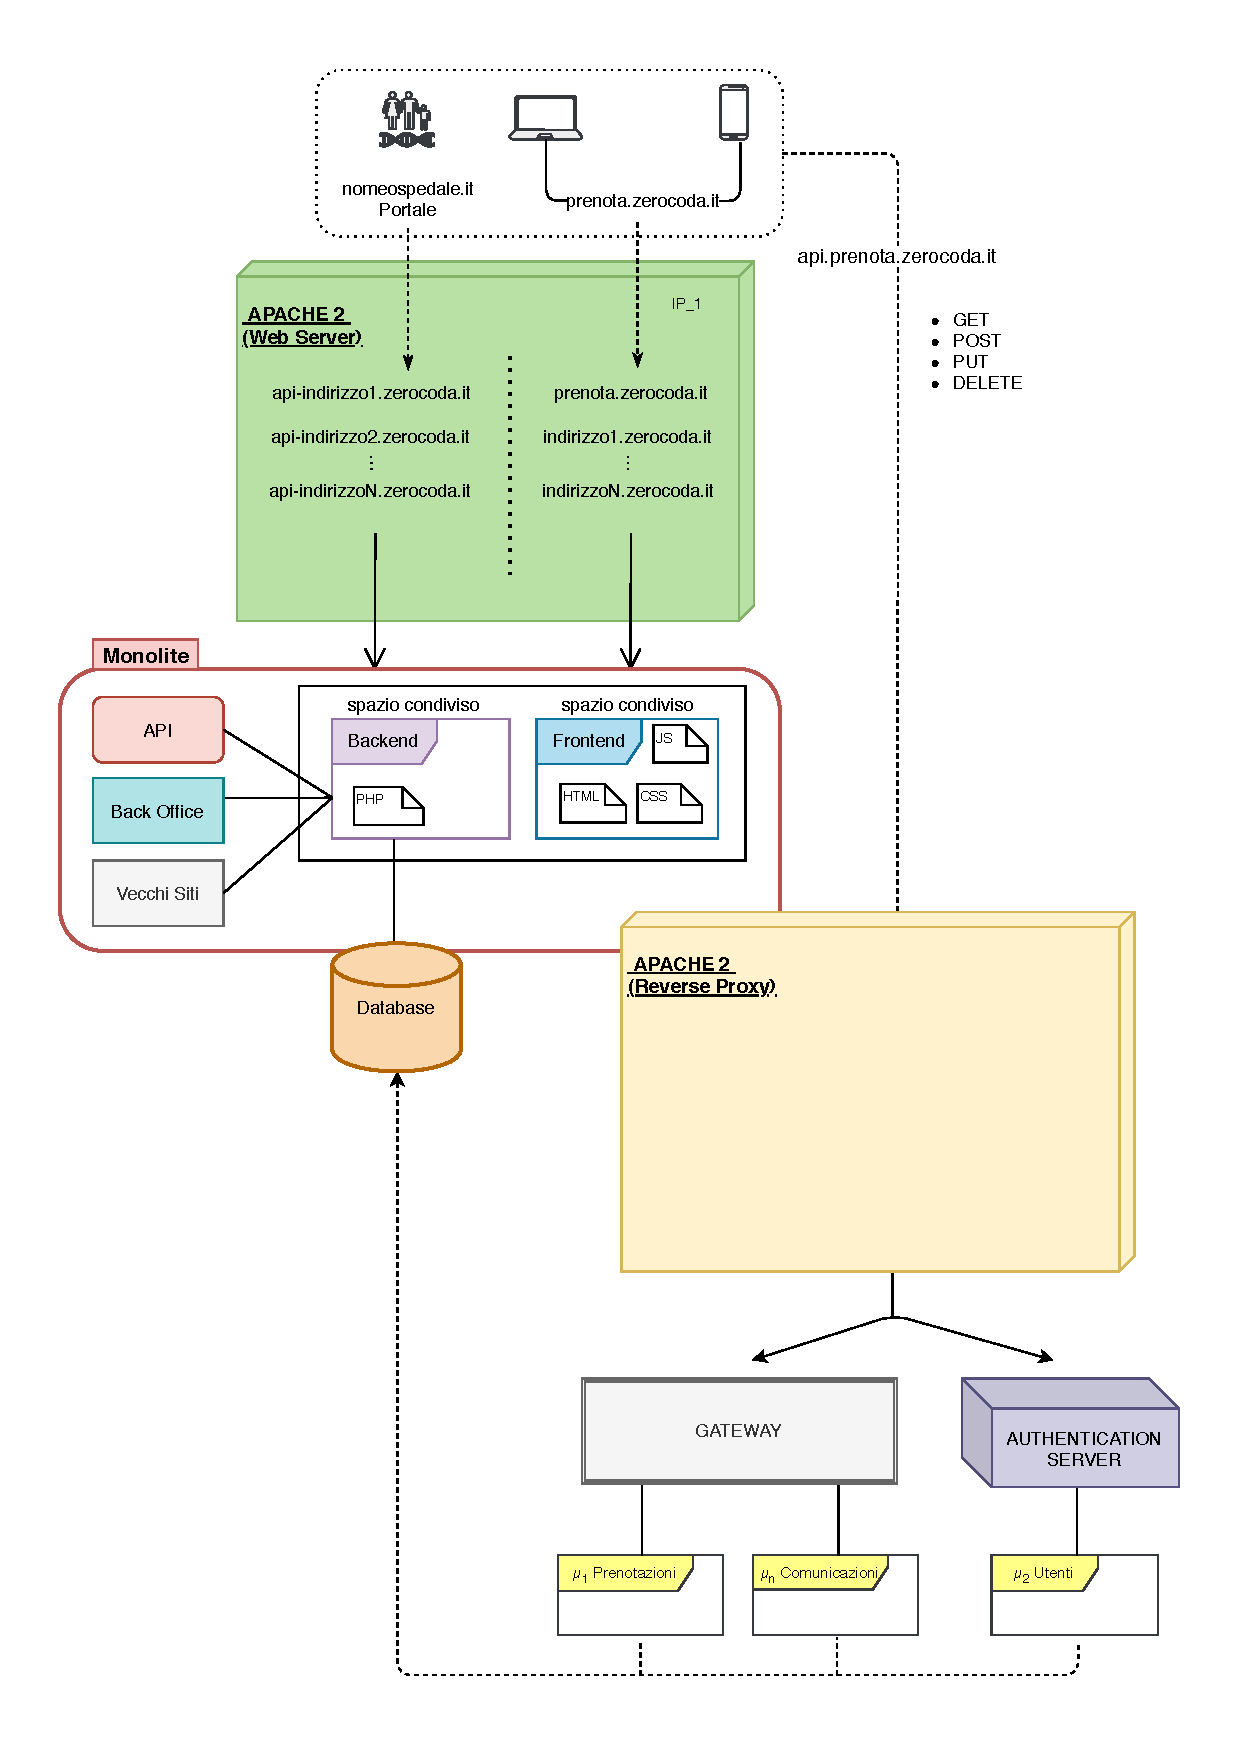
\includegraphics[width=0.98\textwidth]{images/01_new_architecture.pdf}
		\caption{Nuova Architettura del Sistema}
		\label{fig:new_arcchitecture_abstract}
	\end{figure}
	Sulla base di \emph{Zerocoda}, si è deciso di creare un’applicazione analoga per i servizi commerciali: \emph{Zerocoda Retail}. Si tratta di un’esigenza diversa, ma vicina alla precedente. L’idea è già stata sviluppata, nascendo come \emph{fork} di questo software. Il layer di API realizzato costituisce quindi il primo passo sulla strada che porterà alla fusione delle due. Al completamento dell'implementazione delle nuove REST API seguono le successive fasi del refactoring. Queste interessano prima l'\textit{Authentication Server}, il cui sviluppo è cominciato in parallelo a questo progetto, e, in seguito, il frontend, che subirà un leggero restyling finalizzato a migliorare il supporto alle nuove chiamate REST. Nella fase ancora successiva si procederà allo sviluppo del \textit{Communication Server}. Zerocoda offre la possibilità ai propri utenti di essere notificati attraverso email e sms. Questi servizi sono offerti da terzi e permettono all'utente di ricevere aggiornamenti riguardo lo stato della propria prenotazione, o per operazioni di autenticazione. I server sopra citati rappresentano i nuovi microservizi introdotti dal sistema progettato. Poiché il sistema precedente adotta un'architettura monolitica, è necessario scomporre le funzionalità che mette a disposizione e implementarle una per volta. L'ultima parte del refactoring riguarderà il backoffice, e con esso il database, dove il sistema di gestione dei dati verrà completamente rivoluzionato rispetto lo stato attuale. A questa modifica seguiranno le correzioni ai componenti architetturali a cui si è appena fatto riferimento, che sono stati implementati prima di esso. 

   	\end{document}